\chapter[LaTeX]{Ukážky užitočných príkazov v systéme LaTeX}
\label{kap:latex}

V tejto kapitole si ukážeme príklady niektorých užitočných príkazov,
ako napríklad správne používanie tabuliek a obrázkov, číslovanie
matematických výrazov a podobne. Konkrétne príkazy použité v tejto
kapitole nájdete v zdrojovom súbore \verb'latex.tex'.  Všimnite si, že
pre potreby obsahu a hlavičky stránky je v zdrojovom súbore uvedený aj
skrátený názov tejto kapitoly. Ďalšie užitočné príkazy nájdete aj v
kapitole \ref{kap:clenenie}, na ktorú sme sa na tomto mieste odvolali
príkazom \verb'\ref'.

\section{Obrázky}

Vašu prácu ilustrujte vhodnými obrázkami. Pri použití programu
pdflatex je potrebné pripraviť obrázky vo formáte pdf, jpg alebo
png. Vektorové obrázky (napr. eps, svg) je najvhodnejšie skonvertovať
do formátu pdf, napríklad programom Inkscape.

Na vkladanie obrázkov použite prostredie \verb'figure', ktoré obrázok
umiestni na vhodné miesto, väčšinou na vrch alebo spodok stránky a
tiež sa stará o automatické číslovanie obrázkov. Na každý obrázok sa
treba v hlavnom texte odvolať. Napríklad ilustráciu hry Červík vidíme
na obrázku \ref{obr:cursus}. Pri odvolávaní sa na číslo obrázku
používame príkaz \verb'\ref'. Pri vložení alebo zmazaní obrázku tak
nemusíme ručne všetky ostatné obrázky prečíslovať.

\begin{figure}
%vlozenie samotneho obrazku vycentrovaneho a vhodnej velkosti
%obrazok je v subore images/cervik.png
\centerline{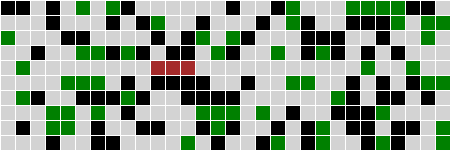
\includegraphics[width=0.4\textwidth]{images/cervik}}
%popis obrazku
\caption[Ukážka hry Červík]{Ukážka hry Červík. Červík je znázornený červenou farbou, voľné políčka sivou, jedlo zelenou a steny čiernou. Hoci tento popis obrázku je dlhší, v zdrojovom texte je aj kratšia verzia, ktorá sa zobrazí v zozname obrázkov.}
%id obrazku, pomocou ktoreho sa budeme na obrazok odvolavat
\label{obr:cursus}
\end{figure}

Podobne tabuľky vkladajte pomocou prostredia \verb'table', pričom
samotnú tabuľku vytvoríte príkazom \verb'tabular'. Každú tabuľku potom
spomeňte aj v hlavnom texte. Napríklad v tabuľke \ref{tab:cas}
vidíme porovnanie časov niekoľkých fiktívnych programov.

\begin{table}
% v tabulke sa popis zvykne davat nad tabulku
\caption[Doba výpočtu a operačná pamäť potrebná na spracovanie vstupu XYZ]{Doba výpočtu a operačná pamäť potrebná na spracovanie vstupu XYZ. V tomto popise môžeme vysvetliť detaily potrebné pre pochopenie údajov v tabuľke.}
%id tabulky
\label{tab:cas}
% tu zacina samotna tabulka
\begin{center}
\begin{tabular}{lrr}
\hline 
Meno programu & Čas (s) & Pamäť (MB) \\
\hline
Môj super program & 25.6 & 120 \\
Speedy 3.1  & 32.1 & 100 \\
VeryOld & 244.1 & 200 \\
\hline
\end{tabular}
\end{center}
\end{table}

V texte môžete tiež potrebovať dlhšie matematické výrazy, ako napríklad tento
\begin{equation}
\sum_{k=0}^n q^k = \frac{q^{n+1}-1}{q-1}.
\label{eq:geom}
\end{equation}
Použitím prostredia \verb'equation' bol tento výraz zarovnaný na stred na
zvláštnom riadku a očíslovaný. Na toto číslo sa tiež môžeme odvolať
príkazom \verb'\ref'. Napríklad rovnica (\ref{eq:geom}) predstavuje súčet 
geometrickej postupnosti.

Napokon, v texte nezabudnite citovať použitú literatúru pomocou príkazu 
\verb'\cite'  Napríklad ďalšie detaily o systéme LaTeX nájdete v knihe od Tobiasa Oetikera a kolektívu \cite{Oetiker2000}.


V tejto kapitole si povieme niečo o jadre práce a o jej členení. V
zdrojovom kóde v súbore \verb'kapitola.tex' nájdenie ukážky použitých
príkazov LaTeXu potrebných na písanie nadpisov a podnadpisov a
číslovaných a nečíslovaných zoznamov. Zvyšok textu tejto kapitoly je
prebratý zo smernice o záverečných prácach \cite[článok 5]{smernica}.

Jadro je hlavná časť školského diela a člení sa na kapitoly,
podkapitoly, odseky a pod., ktoré sa vzostupne číslujú.

\section{Členenie}
Členenie jadra školského diela je určené typom  školského diela. Vo vedeckých 
a odborných prácach má jadro spravidla tieto hlavné časti:
\begin{itemize}
\item  súčasný stav riešenej problematiky doma a v zahraničí,
\item  cieľ práce,
\item  metodika práce a metódy skúmania,
\item  výsledky práce, 
\item  diskusia. 
\end{itemize}

\subsection{Súčasný stav}
V časti súčasný stav riešenej problematiky doma a v zahraničí autor uvádza 
dostupné informácie a poznatky týkajúce sa danej témy. Zdrojom pre spracovanie sú 
aktuálne publikované práce domácich a zahraničných autorov.  Podiel tejto časti práce 
má tvoriť približne 30 \% práce.

\subsection{Cieľ práce}
Časť cieľ práce  školského diela jasne, výstižne a presne charakterizuje predmet 
riešenia. Súčasťou sú aj rozpracované čiastkové ciele, ktoré podmieňujú dosiahnutie 
cieľa hlavného. 

\subsection{Metodika práce a metódy skúmania}
Časť metodika práce a metódy skúmania spravidla obsahuje:
\begin{enumerate}
\item  charakteristiku objektu skúmania,  
\item  pracovné postupy, 
\item  spôsob získavania údajov a ich zdroje, 
\item  použité metódy vyhodnotenia a interpretácie výsledkov,
\item  štatistické metódy.
\end{enumerate}

\subsection{Výsledky práce a diskusia}
Časti výsledky práce a diskusia sú najvýznamnejšími  časťami  školského diela. 
Výsledky (vlastné postoje alebo vlastné riešenia), ku ktorým autor dospel, sa musia 
logicky usporiadať a pri opisovaní sa musia dostatočne zhodnotiť. Zároveň sa 
komentujú všetky skutočnosti a poznatky v konfrontácii s výsledkami iných autorov. 
Výsledky práce a diskusia môžu tvoriť aj jednu samostatnú časť  a spoločne tvoria 
spravidla 30 až 40 \% školského diela.
